\documentclass[9pt]{extarticle}
\title{}
\author{Avinash Iyer}
\date{}
\usepackage[shortlabels]{enumitem}

%font setup
%
%\usepackage{newpxtext,eulerpx}

%paper setup
\usepackage{geometry}
\geometry{letterpaper, portrait, margin=1in}
\usepackage{fancyhdr}

%symbols
\usepackage{amsmath}
\usepackage{amssymb}
\usepackage{mathtools}
\usepackage{hyperref}
\usepackage{gensymb}
\usepackage{multirow,array}

\usepackage[T1]{fontenc}
\usepackage[utf8]{inputenc}

%chemistry stuff
\usepackage[version=4]{mhchem}
\usepackage{chemfig}

%plotting
\usepackage{pgfplots}
\usepackage{tikz}
\tikzset{middleweight/.style={pos = 0.5, fill=white}}
\tikzset{weight/.style={pos = 0.5, fill = white}}
\tikzset{lateweight/.style={pos = 0.75, fill = white}}
\tikzset{earlyweight/.style={pos = 0.25, fill=white}}

%\usepackage{natbib}

%graphics stuff
\usepackage{graphicx}
\graphicspath{ {./images/} }

%code stuff
%when using minted, make sure to add the -shell-escape flag
%you can use lstlisting if you don't want to use minted
%\usepackage{minted}
%\usemintedstyle{pastie}
%\newminted[javacode]{java}{frame=lines,framesep=2mm,linenos=true,fontsize=\footnotesize,tabsize=3,autogobble,}
%\newminted[cppcode]{cpp}{frame=lines,framesep=2mm,linenos=true,fontsize=\footnotesize,tabsize=3,autogobble,}

%\usepackage{listings}
%\usepackage{color}
%\definecolor{dkgreen}{rgb}{0,0.6,0}
%\definecolor{gray}{rgb}{0.5,0.5,0.5}
%\definecolor{mauve}{rgb}{0.58,0,0.82}
%
%\lstset{frame=tb,
%	language=Java,
%	aboveskip=3mm,
%	belowskip=3mm,
%	showstringspaces=false,
%	columns=flexible,
%	basicstyle={\small\ttfamily},
%	numbers=none,
%	numberstyle=\tiny\color{gray},
%	keywordstyle=\color{blue},
%	commentstyle=\color{dkgreen},
%	stringstyle=\color{mauve},
%	breaklines=true,
%	breakatwhitespace=true,
%	tabsize=3
%}
% text + color boxes
\usepackage[most]{tcolorbox}
\tcbuselibrary{breakable}
\newtcolorbox{problem}[1]{colback = white, title = {#1}, breakable}
\newtcolorbox{solution}{colback = white, colframe = black!75!white, title = Solution, breakable}
%including PDFs
%\usepackage{pdfpages}
\setlength{\parindent}{0pt}

\pagestyle{fancy}
\fancyhf{}
\rhead{Avinash Iyer}
\lhead{Applications of Graph Theory: Homework 2}
\newcommand{\card}{\text{card}}
\newcommand{\ran}{\text{ran}}
\newcommand{\N}{\mathbb{N}}
\newcommand{\Q}{\mathbb{Q}}
\newcommand{\Z}{\mathbb{Z}}
\newcommand{\R}{\mathbb{R}}
\begin{document}
  \begin{problem}{6a}
    Show that there is no knight's tour on the $5\times 5$ chessboard.
    \tcblower
    In order to visit all the corners of the $5\times 5$ chessboard, one needs to go along the following cycle:
    \begin{center}
      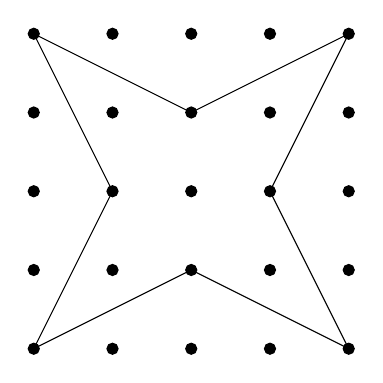
\begin{tikzpicture}
        \foreach \x in {0,1,2,3,4}{
          \foreach \y in {0,1,2,3,4}{
            \filldraw (\x,\y) circle (2pt);
          }
        }
        \draw (0,0) -- (2,1) -- (4,0) -- (3,2) -- (4,4) -- (2,3) -- (0,4) -- (1,2) -- (0,0);
      \end{tikzpicture}
    \end{center}
    If the knight were to visit any of the other squares, it would have to visit one of the center four squares more than once, meaning a knight's tour is impossible.
  \end{problem}
  \begin{problem}{9}
    A graph $G$ of order 20 has the integers $1,2,\dots,20$ as its vertices. Two vertices $i$ and $j$ are adjacent if $i+j$ is odd. Is $G$ Hamiltonian?
    \tcblower
    $G$ is a complete bipartite graph with $2,4,\dots,20$ as one partite set and $1,3,\dots 19$ as another partite set, meaning that a potential Hamiltonian cycle is as follows: $1,2,3,\dots,20,1$.
  \end{problem}
  \begin{problem}{10}
    A graph $G$ of order $n\geq 4$ has $d(v) \geq (n+1)/2$ for each vertex $v$ of $G$.
    \begin{enumerate}[(a)]
      \item Show that $G$ is Hamiltonian.
      \item If $v$ is a vertex of $G$, is $G-v$ Hamiltonian?
    \end{enumerate}
    \tcblower
    \begin{problem}{(a)}
      Let $u,v\in V(G)$. If $u\not\leftrightarrow v$, then $d(u) + d(v) \geq n+1 \geq n$, so by Ore's Theorem, $G$ must be Hamiltonian.\\

      If $u\leftrightarrow v$, then the following cases must hold:
      \begin{enumerate}[(i)]
        \item WLOG, $\exists c\not\leftrightarrow v$, so $d(c) + d(v) \geq n+1 \geq n$, so by Ore's Theorem, $G$ must be Hamiltonian.
        \item $\forall c\leftrightarrow u,~c\leftrightarrow v$, meaning $G$ is complete, and so $G$ is Hamiltonian.
      \end{enumerate}
    \end{problem}
    \begin{problem}{(b)}
      If $v$ is deleted from $G$, the degree of any remaining vertex is either reduced by $1$ or not reduced at all. In either case, the conditions of Ore's Theorem must hold, so $G$ would still be Hamiltonian.
    \end{problem}
  \end{problem}
  \begin{problem}{11}
    Determine whether the following graph is Hamiltonian:
    \begin{center}
      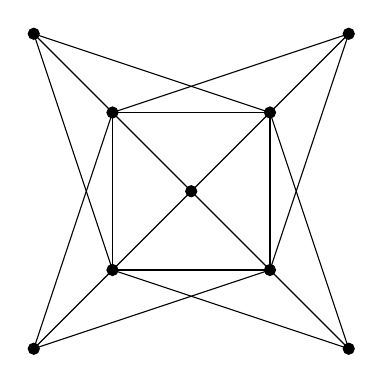
\begin{tikzpicture}
        \foreach \x in {1,-1}{
          \foreach \y in {1,-1}{
            \filldraw (\x,\y) circle (2pt);
          }
        }
        \foreach \x in {2,-2}{
          \foreach \y in {2,-2}{
            \filldraw (\x,\y) circle (2pt);
          }
        }
        \filldraw (0,0) circle (2pt);
        \draw (1,1) -- (1,-1) -- (-1,-1) -- (-1,1) -- cycle;
        \foreach \x in {2,-2}{
          \foreach \y in {2,-2}{
            \draw (0,0) -- (\x,\y);
          }
        }
        \draw (2,2) -- (-1,1);
        \draw (2,2) -- (1,-1);
        \draw (-2,2) -- (1,1);
        \draw (-2,2) -- (-1,-1);
        \draw (2,-2) -- (1,1);
        \draw (2,-2) -- (-1,-1);
        \draw (-2,-2) -- (-1,1);
        \draw (-2,-2) -- (1,-1);
      \end{tikzpicture}
    \end{center}
    \tcblower
    As depicted below, the graph is tripartite.
    \begin{center}
      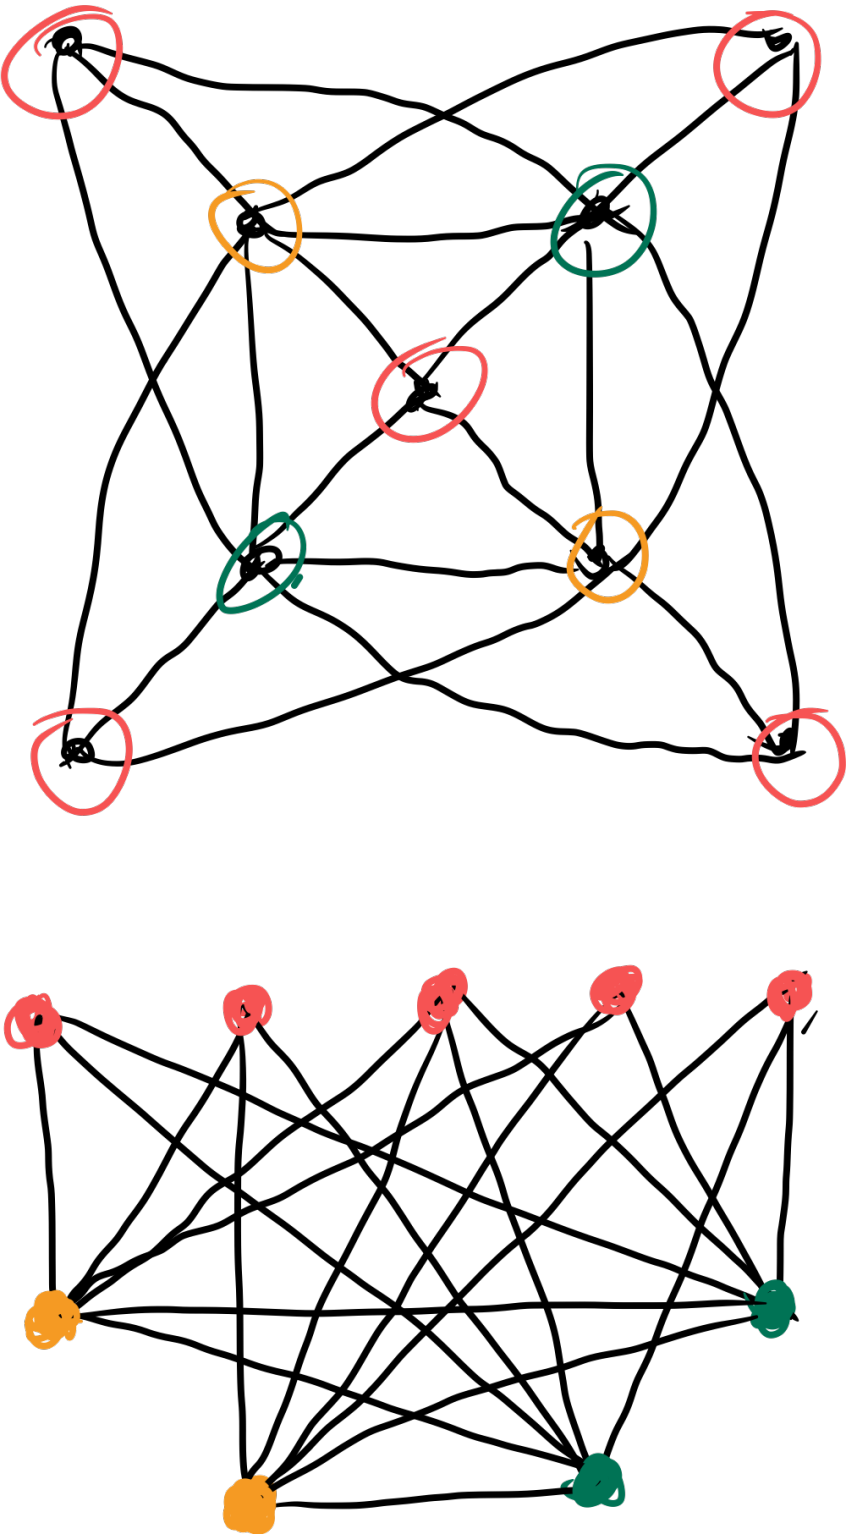
\includegraphics[scale=0.15]{6_11_sol.png}
    \end{center}
    If we delete the orange and green vertices, we will be left with five components (the five solitary vertices above), so by Theorem 6.5, the graph is not Hamiltonian.
  \end{problem}
  \begin{problem}{Extra Problem 1}
    Let $G$ be a graph of order $n\geq 3$, where $\forall v\in G,~d(v) \geq \frac{n}{2}$. Let $P$ be a path in $G$ with longest length.
    \begin{enumerate}[(a)]
      \item Show that $P$ has at least $n/2$ vertices.
      \item Assume there is a cycle $C$ with the same vertices as $P$. Show that $P$ has $n$ vertices.
    \end{enumerate}
    \tcblower
    \begin{problem}{(a)}
      Let $P = (v_1,v_2,\dots,v_k)$ be a path in $G$ with maximum length. Suppose toward contradiction that $|P| < n/2$, meaning $k< n/2$. Then, $\not\exists v_i$ such that $v_i$ is connected to any of $v_1,\dots,v_k$, or else we would be able to extend $P$. Thus, $\forall v\in \{v_1,\dots,v_k\}$, $v$ is only adjacent to other members in $v_1,\dots,v_k$. However, this means that the maximum value $v$ can take is $k-1$, and since $k < n/2$, this means $k-1 < n/2$, or that $v$ would not satisfy one of the conditions of $G$. $\bot$
    \end{problem}
    \begin{problem}{(b)}
      Let $P$ is a path of maximum length in $G$, and $C$ be a cycle in $G$ such that $V(C) = V(P)$. Suppose toward contradiction that $|P| < n$. Then, $\exists v\in G$ such that $\forall v_i\in P,~v\not\leftrightarrow v_i$. However, since $|P| \geq n/2$, as shown earlier, this means $d(v) < n/2$, which is a contradiction.
    \end{problem}
  \end{problem}
  \begin{problem}{Extra Problem 2}
    Prove that the following graph is not Hamiltonian:
    \begin{center}
      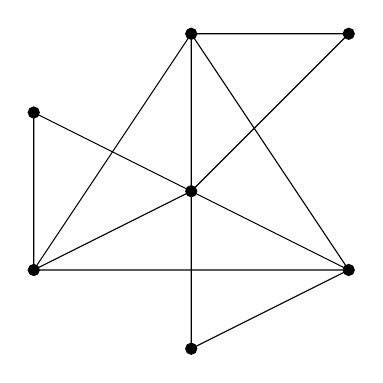
\begin{tikzpicture}
        \filldraw (0,0) circle (2pt)
          (0,2) circle (2pt)
          (0,-2) circle (2pt)
          (2,2) circle (2pt)
          (2,-1) circle (2pt)
          (-2,-1) circle (2pt)
          (-2,1) circle (2pt);
        \draw (0,0) -- (0,2) -- (2,2) -- cycle;
        \draw (0,0) -- (2,-1) -- (0,-2) -- cycle;
        \draw (0,0) -- (-2,-1) -- (-2,1) -- cycle;
        \draw (-2,-1) -- (0,2) -- (2,-1) -- cycle;
      \end{tikzpicture}
    \end{center}
    \tcblower
    All of the degree $2$ vertices in the graph must pass through the center vertex, meaning that a path through this graph cannot pass through all three of the degree $2$ vertices. Thus, the graph is not Hamiltonian.
  \end{problem}
  \begin{problem}{Extra Problem 3}
    The statement of Theorem 6.5 is ambiguous. In the theorem, where it says ``deleting $k$ vertices,'' there are two ways to interpret it:
    \begin{enumerate}[(i)]
      \item Deleting \textit{any} $k$ vertices.
      \item Deleting \textit{some} $k$ vertices.
    \end{enumerate}
    Which one is the correct interpretation?
    \tcblower
    Given that Theorem 6.4 states that for a Hamiltonian graph, deleting \textit{any} $k$ vertices yields a graph with at most $k$ components. The opposite of the statement would most likely be deleting \textit{some} $k$ vertices in a non-Hamiltonian graph yields a graph with more than $k$ vertices.
  \end{problem}
  \begin{problem}{Extra Problem 4}
    The contradiction within the proof is that there are at most $n/2-1$ vertices that are adjacent to $v_k$ (I agree that it could have been phrased better).
  \end{problem}
\end{document}
